\section{Nextflow and nf-core}
\label{sec:nextflow_and_nf-core}
\paragraph{Nextflow} is a workflow management system that enables the
development of reproducible and scalable workflows.
It allows the creation of complex pipelines that can be executed on a variety
of platforms, from local machines to cloud computing environments.
Nextflow uses a domain-specific language (DSL) that simplifies the definition
of workflows and enables the reuse of existing components
\supercite{di_tommaso_nextflow_2017}.
As a result, Nextflow has become a popular tool in the bioinformatics
community.

\begin{figure}[ht]
    \centering

    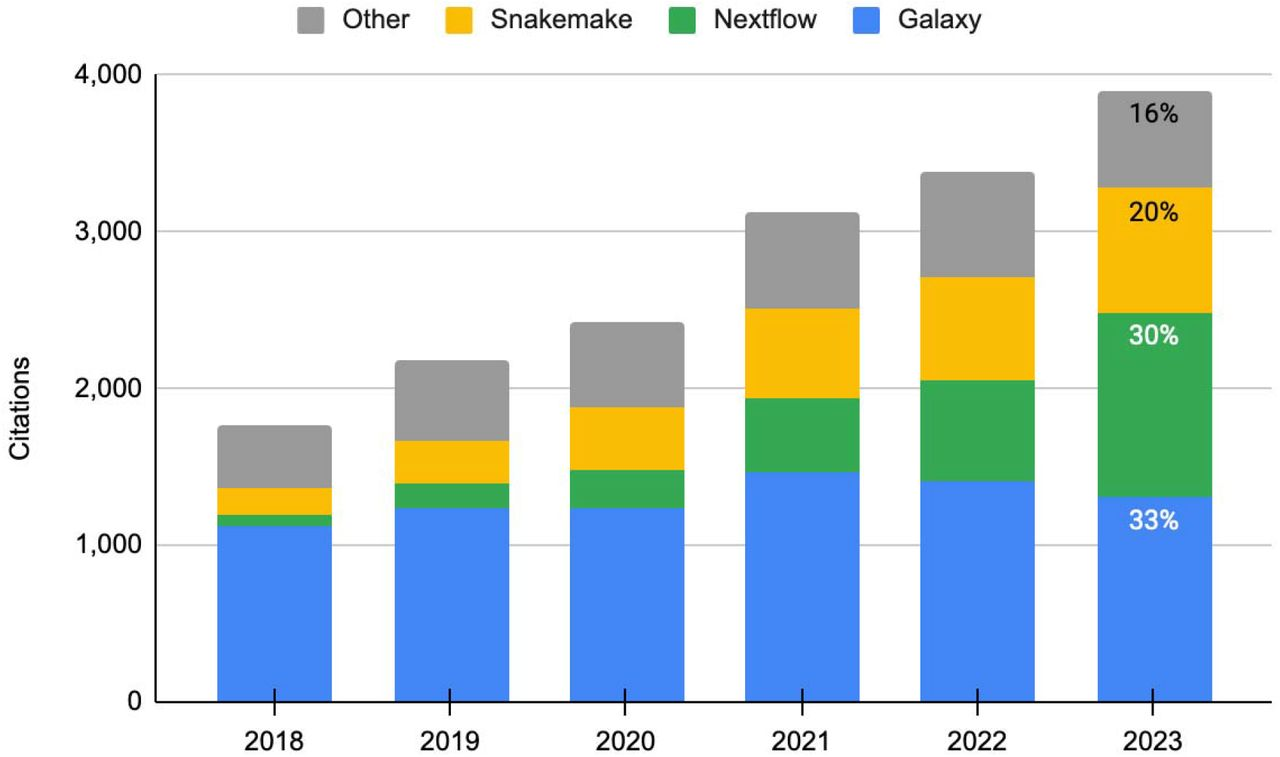
\includegraphics[width=\textwidth]{chapters/3_materials_and_methods/figures/nextflow_usage.jpg}
    \caption{Workflow management systems} % TODO: Add detailed caption
    \label{fig:nextflow_usage}
\end{figure}

As pointed out by Langer et al.
in a recent preprint
\supercite{langer_empowering_2024}, programming-based workflow systems like
Nextflow and Snakemake have gained popularity during the last years, while
GUI-based systems like Galaxy have lost ground.
Furthermore, Nextflow has been the fastest growing workflow system in the last
years, with a remarkable 30 percent share of citations in 2023
(\cref{fig:nextflow_usage}).
The authors mostly attribute this to the great quality of the pipelines curated
by the nf-core community
\supercite{langer_empowering_2024,grayson_automatic_2023}.

\paragraph{nf-core} is a community-driven project that provides a collection of
high-quality, reproducible, and scalable Nextflow pipelines.
These pipelines cover a wide range of bioinformatics applications, from RNA-seq
and ChIP-seq to single-cell RNA-seq and metagenomics
\supercite{ewels_nf-core_2020}.
The community maintains a collection of reusable components, so that developers
can utilize them to speed up the development of new pipelines.
The nf-core project also provides guidelines for best practices in pipeline
development, ensuring that the resulting workflows are robust, efficient, and
easy to use \supercite{ewels_nf-core_2020}.